
\section{Pipeline}
We describe the pipeline $p$ that we run on each text $T$. The pipeline
consists of multiple natural language annotators mentioned in 
\citep{manning2014stanford} that we run in 
the sequence outlined below.

\subsection{Tokenizer}
The tokenizer takes the utterances $u_{1:n}$ and outputs a tuple of
each word in $u_{1:n}$. For example, the tokenizer would transform
the sentence \nl{He'll travel to Minneapolis} to the tuple
\begin{center}
  (\nl{He}, \nl{'ll}, \nl{travel}, \nl{to}, \nl{Minneapolis})
\end{center}
\subsection{Sentence Splitter}
Given the tokens of the utterances $u_{1:n}$, the sentence splitter outputs
a tuple of the sentences $(u_1,\dots,u_n)$. This is necessary
for the tasks below because they operate at the sentence level.

\subsection{Part of Speech}

\begin{figure}
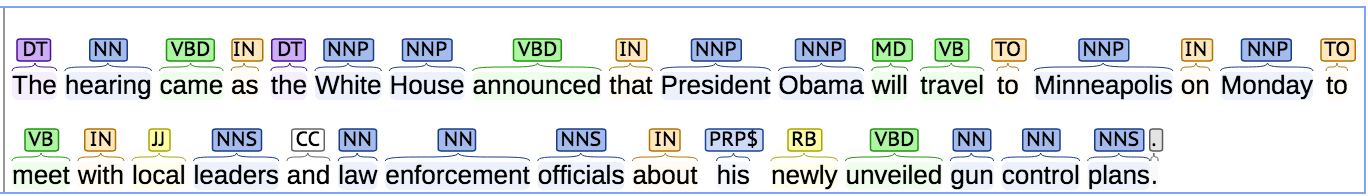
\includegraphics[scale=0.33]{figures/pos.png}
\caption{
\label{fig:pos}
Part of Speech tags for $u_1$.
}
\end{figure}

We run the Stanford Part of Speech (POS) tagger \citep{toutanova2003tagger}
on each utterance $(u_1,\dots,u_n)$. The tagger uses the Penn Treebank
POS tag set. For each utterance $u_i$, the
tagger outputs a tuple of tags $t=(t_1,\dots,t_m)$, where the 
tag $t_j$ corresponds to token $j$ in utterance $i$.

\subsection{Lemmatizer}
The lemmatizer operates on a token-by-token basis, and 
produces a canonical representation for each token. For 
example, the lemmatizer would modify the utterance
\nl{He went to the better team.} to 
\nl{He go to the good team.}

\subsection{Named Entity Recognition}

\begin{figure}
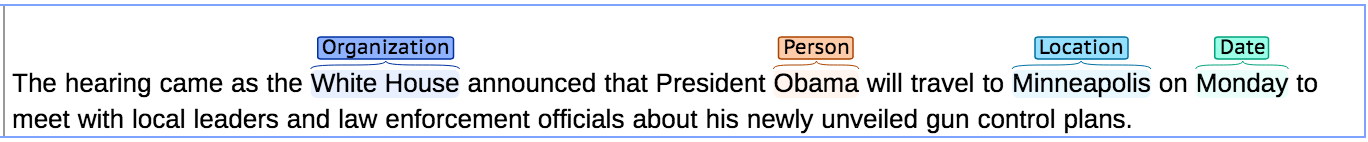
\includegraphics[scale=0.33]{figures/ner.png}
\caption{
\label{fig:ner}
Named Entity Recognition for $u_1$.
}
\end{figure}

Next, we run the Stanford Named Entity Recognition (NER)
annotator on the sentences \citep{finkel2005incorporating}. The annotator is
based on a Conditional-Random Field, and
classifies tokens into one of four categories: People, Location, Organization, Misc.

\subsection{Dependency Parse}

\begin{figure}
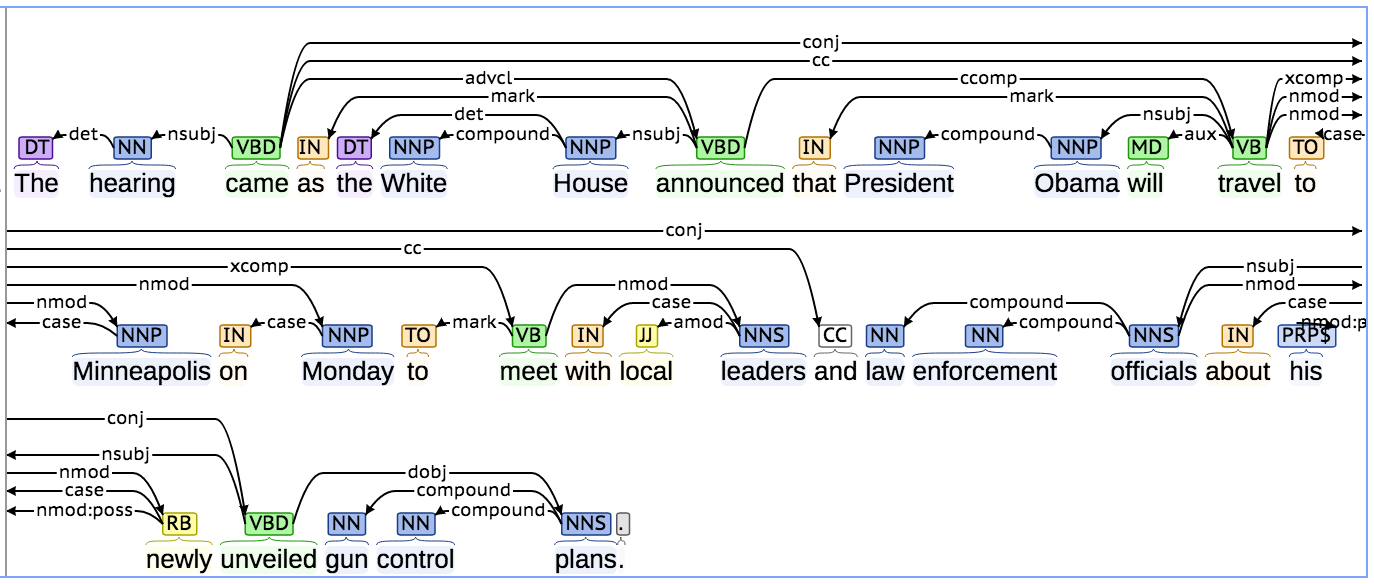
\includegraphics[scale=0.33]{figures/dep.png}
\caption{
\label{fig:dep}
Dependency parse for $u_1$.
}
\end{figure}

A dependency parse represents the relationships between words
in an utterance. This is useful for finding the subject and 
the object in a relation triple. We run Stanford's Neural 
Network Dependency Parser on each utterance $(u_1,\dots,u_n)$
\citep{chen2014nndep}.
\subsection{Mention Resolver}
We use the Stanford Mention Resolver to collapse contiguous
named entities into one. For example, the NER annotator would
label both tokens in \nl{Barack Obama} as Persons, when in reality,
there is only one person. The mention annotator collapses the
\nl{Barack} and \nl{Obama} entities into one entity.

\subsection{Natural Logic}
The Stanford Natural Logic annotator finds
quantifiers for each utterance. For each token,
the annotator ascribes a polarity (either affirmative
or negative).
More information can be found at 
\url{http://nlp.stanford.edu/projects/natlog.shtml}.
\subsection{Coreference Resolution}

\begin{figure}
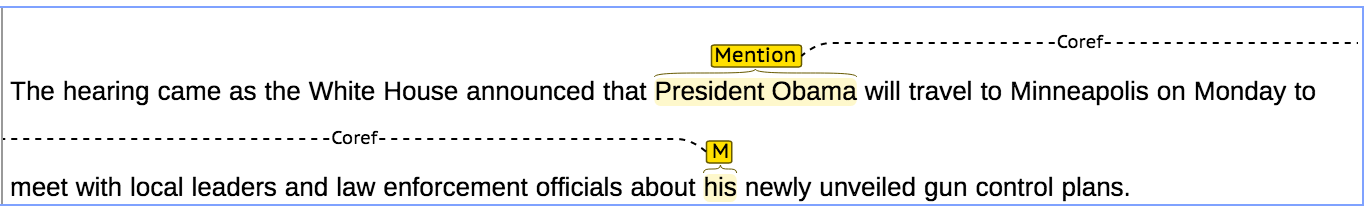
\includegraphics[scale=0.33]{figures/coref.png}
\caption{
\label{fig:coref}
Coreference resolution for $u_1$.
}
\end{figure}

We use the Stanford Statistical Coreference system implemented by
\citet{clark2015coref}. The annotator outputs a directed graph
which encodes the reference relationships between mentions in 
$(u_1,\dots,u_n)$. For example, in $u_1$ given above, it would
recognize that the word \nl{his} in \nl{\dots his newly unveiled \dots}
refers to Barack Obama.

\section{Relation Extractor}
After generating the annotation $A$ for a text $T$, we use our 
extractor $e$ to extract relation triples $R=e(A,T)$. For this 
step, we use the OpenIE system developed by \citet{angeli2015openie}, and
limit the maximum number of entailments taken per clause to 100 entailments.
This is the lowest recommended value that the system recommends, which we
chose to reduce the computational power required.
\rl{Have example sentence and the relations parsed from it}.

\subsection{With Coreference Resolution}


\citet{fader11reverb}
